El \textbf{Border Gateway Protocol (BGP)} es el protocolo de enrutamiento estándar que permite la interconexión de los Sistemas Autónomos (AS) en la Internet global. A diferencia de los protocolos de puerta de enlace interior (IGP), BGP no busca simplemente el camino físico más corto, sino que actúa como un sistema de intercambio de políticas que garantiza la accesibilidad y la estabilidad de la red a gran escala.

\subsection{Características Generales del Protocolo BGP}

BGP es un protocolo único que se distingue por su enfoque en la \textbf{alcanzabilidad} y el control administrativo. Sus características fundamentales incluyen:

\begin{itemize}
	\item \textbf{Algoritmo de Vector de Ruta (\textit{Path-Vector}):} A diferencia de los algoritmos de vector-distancia o estado de enlace, BGP registra la lista completa de Sistemas Autónomos que un paquete debe atravesar. Esto elimina de raíz la posibilidad de bucles de enrutamiento.
	\item \textbf{Transporte sobre TCP:} BGP utiliza el puerto 179 de TCP. Al delegar la fiabilidad y el control de flujo a TCP, el protocolo no necesita mecanismos propios de retransmisión o fragmentación.
	\item \textbf{Soporte de CIDR (\textit{Classless Inter-Domain Routing}):} BGP fue el motor que permitió la transición hacia el enrutamiento "sin clase". CIDR elimina la rígida división de redes en clases (A, B, C), permitiendo una asignación de direcciones mucho más eficiente mediante el uso de prefijos de longitud variable.
	\item \textbf{Actualizaciones Incrementales:} Tras un intercambio inicial de la tabla de rutas completa, los pares BGP solo envían "deltas" (cambios específicos), lo que minimiza el consumo de ancho de banda.
	\item \textbf{iBGP y eBGP:} Se utiliza \textbf{eBGP} para la comunicación entre diferentes AS, mientras que \textbf{iBGP} permite que los enrutadores internos de un mismo AS coordinen la información aprendida del exterior de forma coherente.
\end{itemize} 

\subsection{Tipos de Mensajes BGP}

La operación de BGP se gestiona a través de cinco tipos de mensajes principales, protegidos por un encabezado común de 19 octetos:

\begin{enumerate}
	\item \textbf{OPEN:} Inicia la sesión. Incluye el número de AS, la versión del protocolo y el identificador BGP (generalmente la dirección IP más alta del router).
	\item \textbf{UPDATE:} Es el corazón del protocolo. Anuncia nuevas rutas o retira las obsoletas. Es aquí donde se aplica la compresión CIDR, enviando el par (longitud de máscara, prefijo) de forma optimizada.
	\item \textbf{KEEPALIVE:} Mensajes cortos (solo el encabezado) enviados periódicamente para confirmar que el par sigue operativo, dado que TCP no detecta fallos de enlace de forma inmediata si no hay tráfico.
	\item \textbf{NOTIFICATION:} Se utiliza para informar errores críticos. Tras su envío, la conexión TCP se cierra inmediatamente para preservar la integridad de las tablas de rutas.
	\item \textbf{ROUTE-REFRESH:} Permite solicitar a un par que reenvíe sus anuncios de ruta sin necesidad de reiniciar la sesión TCP.
\end{enumerate}

\subsection{Estructura de un Mensaje UPDATE}

El mensaje UPDATE es la unidad de intercambio de información de accesibilidad. Para maximizar la eficiencia, BGP factoriza los \textbf{Atributos de Ruta}: todos los destinos listados en un único mensaje comparten los mismos metadatos (como el AS-PATH o el Next-Hop).

\begin{figure}[H]
	\centering
	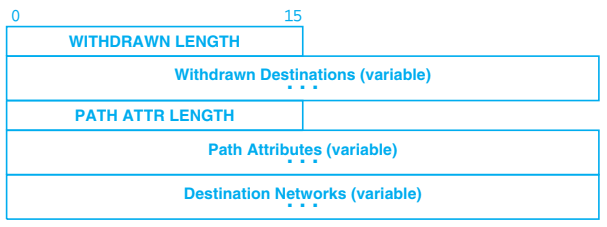
\includegraphics[width=0.6\textwidth]{img/bgpupdate.png}
	\caption{Estructura del mensaje BGP UPDATE con campos de longitud variable.}
	\label{fig:grafico13}
\end{figure}

En la sección de destinos, BGP aplica una técnica de empaquetado compacto para el direccionamiento CIDR: se envía un octeto con la longitud del prefijo seguido únicamente de los octetos significativos de la dirección IP. Por ejemplo, una red /16 solo consume 2 octetos de dirección en el mensaje, reduciendo drásticamente el tamaño de las actualizaciones globales.

\subsection{Atributos de Ruta y Toma de Decisiones}

Los Atributos de Ruta son metadatos esenciales que BGP adjunta a cada anuncio de red para guiar el proceso de selección de rutas. Los más críticos son:

\begin{itemize}
	\item \textbf{AS-PATH (Atributo 2):} Una lista ordenada de los ASN que la ruta ha recorrido. Si un router detecta su propio ASN en la lista, descarta el anuncio, evitando bucles.
	\item \textbf{NEXT-HOP (Atributo 3):} Indica la dirección IP del router que debe utilizarse para alcanzar el destino. En BGP, este "siguiente salto" no es necesariamente un vecino directo, sino la puerta de entrada al siguiente AS.
	\item \textbf{LOCAL-PREF:} Utilizado internamente en un AS para preferir una ruta de salida sobre otra.
	\item \textbf{MED (\textit{Multi-Exit Discriminator}):} Permite a un AS sugerir a sus vecinos cuál es el punto de entrada preferido hacia su red cuando existen múltiples conexiones.
\end{itemize}
